In their \textit{Stochastic Gradient Hamiltonian Monte Carlo}, Chen, Fox, and Guestrin propose using a subset $\tilde{\mathcal{D}}$ of the entire dataset $\mathcal{D}$ to compute
\begin{equation*}
	\Delta\tilde{U}(\theta)=-\frac{|\mathcal{D}|}{|\tilde{\mathcal{D}}|}\sum_{x\in\tilde{\mathcal{D}}}\Delta\log p(x|\theta) - \Delta\log p(\theta)
\end{equation*}
which can then be used in the Hamiltonian Monte Carlo equations in the stead of the gradient $\Delta U(\theta)$.

Logistic regression assigns the probability of success to a dichotomous response variable

\begin{equation*}
	\prob{y_i=1|\bm{x}_{i},\bm{\beta}}=\frac{\exp\braces{\bm{x}_i^T\bm{\beta}}}{1+\exp\braces{\bm{x}_i^T\bm{\beta}}}
\end{equation*}

where $\bm{x}_i$ is a vector of length $p$ covariates for data point $i$ and $\bm{\beta}$ is a vector of regression coefficients of length $p$. In a Bayesian framework, we would assign the a prior distribution on our unknown parameters $P(\bm{\beta})\sim\mathcal{N}(0, \sigma^2)$ where, for the purposes of our project, $\sigma^2$ is known. The corresponding posterior will be proportional to $P(\theta)\prod_{i=1}^n\prob{y_i|\bm{x}_i,\bm{\beta}}$, which would give us the potential energy function
\begin{equation*}
U(\bm{\beta})=-\log\left[P(\bm{\beta})\right] - \sum_{i=1}^n\log\left[\prob{y_i|\bm{x}_i,\bm{\beta}}\right]=\sum_{j=1}^p\frac{\beta_j^2}{2\sigma^2}-\sum_{i=1}^n\left[y_i(\bm{x}_i^T\bm{\beta})-\log(1+\exp\braces{\bm{x}_i^T\bm{\beta}})\right]
\end{equation*}
and gradient components
\begin{equation*}
\frac{\partial U}{\partial \beta_j}=\frac{\beta_j}{\sigma^2}-\sum_{i=1}^{n}x_{ij}\left[y_i-\frac{\exp\braces{\bm{x}_i^T\bm{\beta}}}{1+\exp\braces{\bm{x}_i^T\bm{\beta}}}\right]. 
\end{equation*}
In practice, the stochastic gradient is noisy since it is an approximation of the gradient. The paper suggests introducing a friction term to the momentum to dampen the movement of the chain. The algorithm will take a user specified friction term $C$ that is element-wise bigger than the noise model $B$. The noise model is unknown but can be set to zero for simplicity. The final algorithm will be:

\begin{algorithm}[H]
	\KwIn{Starting position $\theta^{(1)}$ and step size $\epsilon$.}
	\For{t=1, 2, \dots} {
		Sample momentum $r^{(1)}\sim\mathcal{N}(0, M)$\\
		\For{i=1,\dots,m} {
			$\theta_i=\theta_{i-1}+\epsilon M^{-1}r_{i-1}$\\
			$r_i = r_{i-1} + \epsilon \Delta\tilde{U}(\theta_i)-\epsilon C M^{-1}r_{i-1}+\mathcal{N}(0, 2(C-\hat{B})\epsilon)$\\
		}
		$(\theta^{t+1}, r^{t+1})=(\theta_m, r_m)$\\
	}
\end{algorithm}

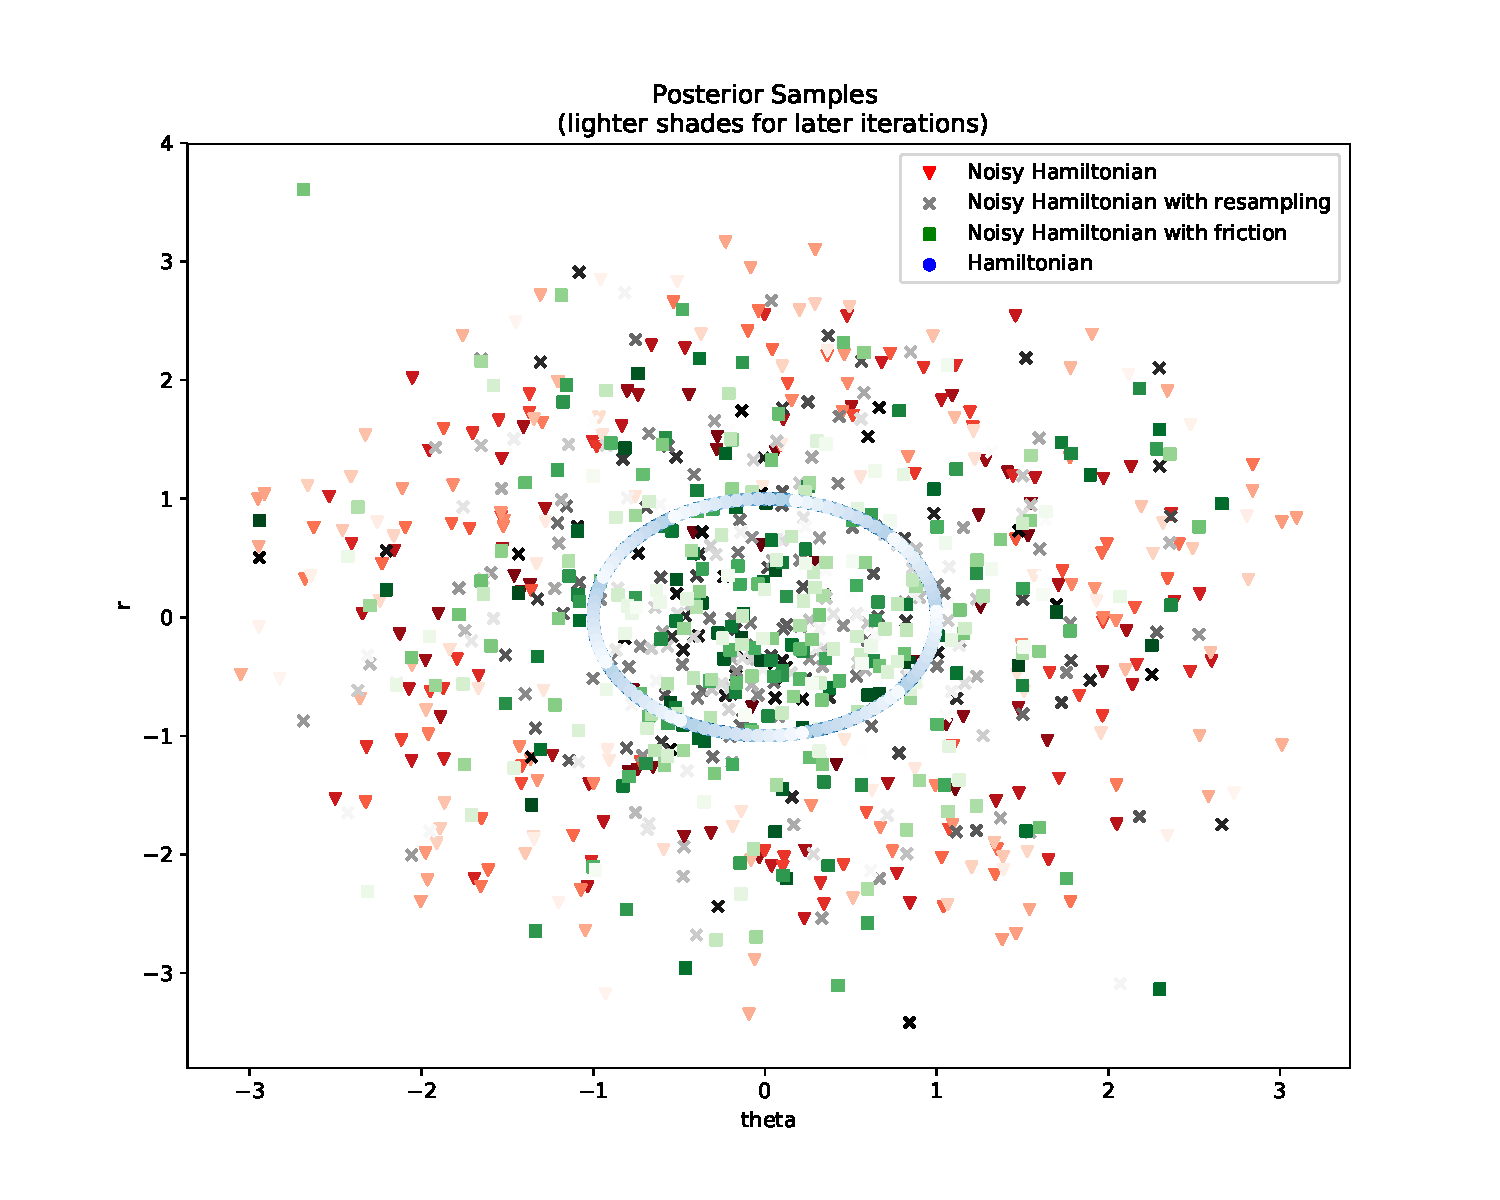
\includegraphics[width=\textwidth]{posterior_samples.pdf}